% Generated by tools/analysis/analyze.py; do not edit by hand.
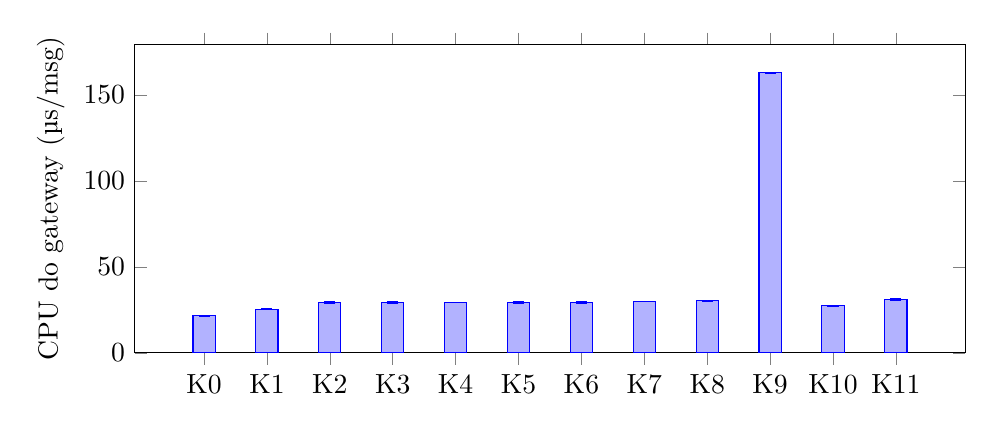
\begin{tikzpicture}
  \begin{axis}[width=\linewidth, height=5.5cm, ybar, bar width=8pt,
      ylabel={CPU do gateway (µs/msg)}, xtick={0,...,11},
      xticklabels={K0,K1,K2,K3,K4,K5,K6,K7,K8,K9,K10,K11}, ymin=0,
      error bars/y dir=both, error bars/y explicit]
    \addplot+[error bars/.cd, y dir=both, y explicit] coordinates {
      (0,21.720) +- (0,0) -= (0,0.240) += (0,0.210)
      (1,25.400) +- (0,0) -= (0,0.320) += (0,0.230)
      (2,29.325) +- (0,0) -= (0,0.585) += (0,0.270)
      (3,29.440) +- (0,0) -= (0,0.390) += (0,0.310)
      (4,29.330) +- (0,0) -= (0,0.210) += (0,0.180)
      (5,29.440) +- (0,0) -= (0,0.550) += (0,0.230)
      (6,29.365) +- (0,0) -= (0,0.595) += (0,0.535)
      (7,29.955) +- (0,0) -= (0,0.260) += (0,0.115)
      (8,30.460) +- (0,0) -= (0,0.505) += (0,0.245)
      (9,162.765) +- (0,0) -= (0,0.230) += (0,0.270)
      (10,27.595) +- (0,0) -= (0,0.350) += (0,0.160)
      (11,30.950) +- (0,0) -= (0,0.270) += (0,0.560)
    };
  \end{axis}
\end{tikzpicture}
